\documentclass[]{article}
\usepackage{float,url,multirow}
\usepackage[nottoc,numbib]{tocbibind}
\usepackage{graphicx} 
\graphicspath{{./figs/}}

%opening
\title{Extinctions}
\author{Simon Crase}

\begin{document}

\maketitle

\begin{abstract}
I found that \cite{Wilensky:1997} exhibits behaviour that I did not expect: it appears stable, but when I increased the speed at which grass regrows slightly, regrowth time=20, the model ran for some 1,200,000 generations, then the wolves become extinct suddenly--Figure \ref{fig:wsg}. I started wondering whether there is some link between diversity and stability.
\end{abstract}

\begin{figure}[b]
	\centering
	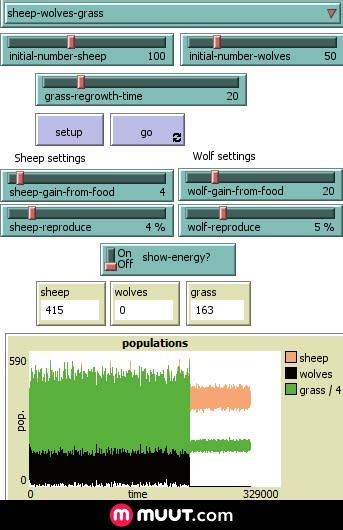
\includegraphics[width=0.5\linewidth]{wsg20.jpg}
	\caption{Wolves Sheep Grass. This run crashes after a couple of hundres thousand generations, but I have observed over 1,200,000. Notice that the crash is very sudden.}
	\label{fig:wsg}
\end{figure}

\section{What part of phenomenon would you like to model?}

\begin{enumerate}
	\item Natural Selection
	\item Stability/Extinction
\end{enumerate}

\section{What are the principal types of agents involved in this phenomenon?}

\begin{enumerate}
	\item Plants
	\item Primary, Secondary, and Tertiary Consumers
\end{enumerate}

\section{What properties do these agents have?}

\begin{enumerate}
	\item Energy
\end{enumerate}

\section{What actions (or behaviours) can these agents take?}

\begin{enumerate}
	\item Plants
	\begin{enumerate}
		\item Grow
	\end{enumerate}	
	\item Primary, Secondary, and Tertiary Consumers
	\begin{enumerate}
		\item Breed
		\item Feed
		\item Die
	\end{enumerate}
\end{enumerate}


\section{If the agents have goals, what are their goals?}

Make as many copies of itself as possible

\section{Agents operate in what kind of environment?}
\section{How do agents interact with environment?}

\medskip

\bibliographystyle{unsrt}
\bibliography{../complexity}

\end{document}
